% Mission elements section
% File: sections/mission_elements.tex
\documentclass[../main.tex]{subfiles}

\begin{document}

\section{Mission elements}\label{mission-elements}
TBD

\subsection{Mission description}\label{mission-description}

MARSNET is a dedicated telecommunication and navigation relay
constellation designed to provide continuous, high-bandwidth, and low-latency
communication coverage for human and robotic exploration on Mars. The network
will consist of a series of orbiters strategically placed in highly elliptical
and areostationary orbits, ensuring global surface coverage and reliable links
between Mars and Earth.

\subsubsection*{Mission Objectives:}

\begin{enumerate}[left=0pt, label=\arabic*., itemsep=2pt, topsep=2pt]
    \item \textbf{Enable Human Exploration:} Seamless voice, video, and data transmission for astronauts, including polar and high-latitude regions.
    \item \textbf{Global Surface Connectivity:} Redundant communications backbone for rovers, habitats, drones, and mobile assets.
    \item \textbf{Earth-Mars Link Reliability:} Continuous interplanetary data flow with adaptive bandwidth for science, telemetry, and emergency channels.
    \item \textbf{Navigation Support:} Precise positioning and timing services for surface and aerial vehicles (Mars-analog to GPS).
    \item \textbf{Scalability for Expansion:} Modular, evolvable network architecture supporting future settlements and missions.
\end{enumerate}

\subsubsection*{Mission Architecture:}

\begin{enumerate}[left=0pt, label=\arabic*., itemsep=2pt, topsep=2pt]
    \item \textbf{Core Constellation:} Three to five relay satellites in areostationary orbit for persistent equatorial and mid-latitude coverage.
    \item \textbf{Supplementary Satellites:} Highly elliptical and polar orbit relays for polar coverage and redundancy during dust storms.
    \item \textbf{High-Gain Mars-Earth Gateway:} Satellites with optical and radio high-gain antennas maintaining a robust link to Earth's Deep Space Network.
    \item \textbf{Inter-Satellite Links:} Crosslink capability enabling dynamic routing of data around outages, creating a true network.
    \item \textbf{Strategic Importance:} MARSNET provides global communication and navigation, removing critical bottlenecks for surface operations and scientific return, ensuring safe, coordinated, and efficient exploration.
\end{enumerate}
\newpage

\subsection{Requirements}\label{requirements}

TBD

% Requirements table and instructions

\emph{Create at least 9 different requirements from a `ECSS Requirement
categories'' perspective, and 8 different requirements from a `Product
Breakdown Structure (PBS)' perspective. Note that this can be combined,
so you could only have 9 requirements in total if you find the right
combinations. Also include the type (key, killer, driving, normal), the
rationale, the verification method (Inspection, Demonstration, Test,
Analysis, By similarity, Simulation and modeling (Design)) and if
applicable, an ECSS document reference.}

\textbf{Reference documents}
\begin{table}[htp]
\centering
% \renewcommand{\arraystretch}{1.2} % row height
\begin{tabularx}{\textwidth}{|p{0.6cm}|X|p{1.5cm}|p{2cm}|p{1cm}|p{2cm}|p{1.2cm}|p{1.4cm}|}
\hline
Req. ID & Description & Rationale & ECSS Req. Category & Type & Applicable PBS level/item & V\&V method & ECSS doc. reference \\
\hline
& & & & & & & \\
\hline
& & & & & & & \\
\hline
& & & & & & & \\
\hline
& & & & & & & \\
\hline
& & & & & & & \\
\hline
& & & & & & & \\
\hline
& & & & & & & \\
\hline
\end{tabularx}
\end{table}

\subsection{Concept designs}\label{concept-designs}

TBD

\subsection{System and subsystem level trade-offs leading to final
concept
design}\label{trade-offs}

TBD

\subsection{Description of system
elements}\label{description-of-system-elements}

TBD

\newpage
\thispagestyle{noheader}
\newgeometry{
    headheight=0pt,
    headsep=0pt,
    bottom=2cm,
    left=2.5cm,
    right=2.5cm,
    top=2cm
}

\begin{landscape}
\subsection{Product Breakdown Structure
(PBS)}\label{pbs}

\resizebox{\linewidth}{!}{%
\begin{forest}
  numbered,
  start label=1,
  [MARSNET Mission% Level 1
    [Space Segment % Level 2
      [Relay Satellites \\(Areostationary) % Level 3
        % [Bus Subsystems % Level 4
        %   [Power \\ Thermal \\ ADCS \\ Propulsion \\ OBDH \\ Structure \\ Communications] % Level 5
        % ]
        % [Bus Subsystems
        %   [Power]
        %   [Thermal]
        %   [ADCS]
        %   [Propulsion]
        %   [OBDH]
        %   [Structure]
        %   [Communications]
        % ]
        % [Payload Suite % Level 4
        %   [High-Gain \\Antenna System] % Level 5
        %   [Optical \\Communication \\Terminal] % Level 5
        %   [Inter-satellite \\Crosslink \\Transceiver] % Level 5
        % ]
        % [Payload Suite % Level 4
          [High-Gain \\Antenna \\System % Level 5
            [Ka-band \\Reflector \\Antenna % Level 6
              [Reflector \\Surface \\Panels]
              [Support Truss/\\Backstructure]
              [Surface \\Deployment \\Mechanism]
            ]
            [S-band / X-band \\Feed Assembly % Level 6
              [Feed Horn]
              [Polarizer / \\Orthomode \\Transducer]
              [Waveguide \\Assembly]
              [Low-Noise \\Amplifier]
              [High-Power \\Amplifier]
            ]
            [Gimbal \& Pointing \\Mechanism]
          ]
          [Optical \\Communication \\Terminal % Level 5
            [Laser \\Transmitter \\Unit]
            [Optical \\Telescope \\Assembly]
            [Acquisition \& \\Tracking \\Sensor]
            [Detector / \\Receiver \\Module]
          ]
          [Inter-satellite \\Crosslink \\Transceiver % Level 5
            [Crosslink \\RF Antenna]
            [Crosslink \\Transceiver \\Electronics]
            [Pointing \& Control \\Interface]
          ]
          % [Timing / Navigation Payload (optional) % Level 5
          %   [Atomic Clock Unit]
          %   [Frequency Reference Oscillator]
          %   [Timing Distribution Electronics]
          % ]
        % ]
      ]
      [Relay Satellites \\(Polar Orbiters)]
      [Inter-satellite \\Link System]
    ]
    [Ground Segment % Level 2
      [Earth Ground \\Stations \\(DSN interface)
      %   [Antenna Systems]
      %   [Tracking \& \\Telemetry \\Subsystems]
      %   [Data Processing\\ Subsystems]
      ]
      [Mission \\Operations \\Center]
    ]
    [Launcher Segment % Level 2
      [Launch Vehicle(s)
      %   [Payload \\Fairing]
      %   [Upper Stage \\Adapter]
      %   [Guidance \& \\Control \\Subsystems]
      ]
      [Integration \\ Facilities]
    ]
    [User Segment % Level 2
      [Mars Surface Assets
        [Surface Comm \\Modules]
        [Portable \\Terminals]
        [Rover/Habitat \\Relay \\Interfaces]
      ]
    ]
  ]
\end{forest}}
\end{landscape}

\restoregeometry
\newpage

TBD

\emph{Below is an example of an 8 levels PBS with generic names in the
boxes. Replace the names with items from your chose concept design, and
preferably also the system and subsystem that you do a trade-off for.
Give the items a unique number that you can also insert in the
requirements table.}

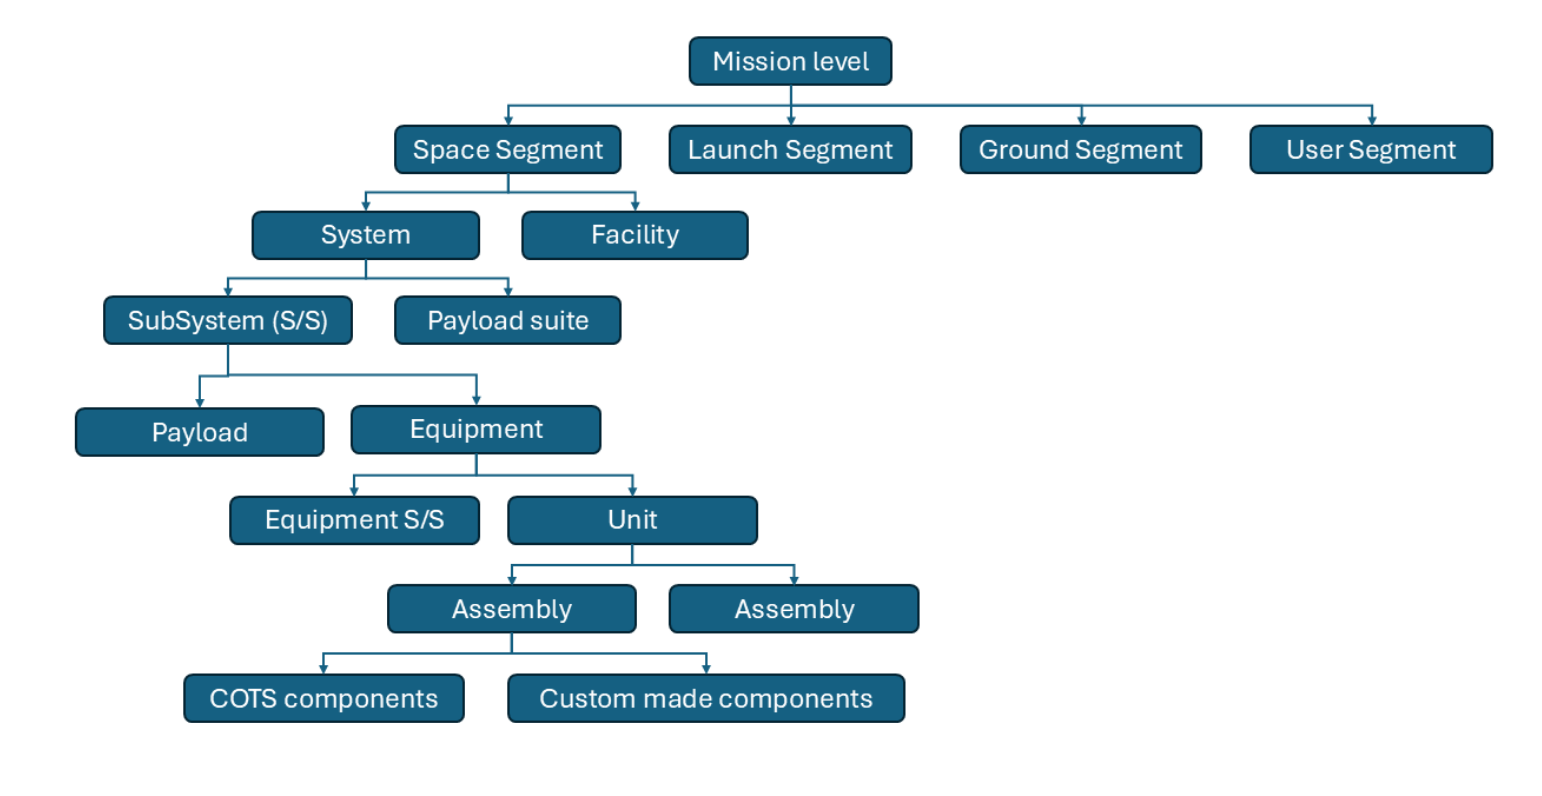
\includegraphics[width=6.28264in,height=3.53403in]{media/Product Breakdown Structure.png}

\subsection{Verification and Validation of
requirements}\label{verification-and-validation}

TBD

\end{document}
